\section{Mapping from Low to High}
\label{sec:challenges}

%[commented by MRA] We discuss how to use low-level performance metrics collected from distributed components to build an accurate end-to-end performance model for a distributed storage system in the SDS environment.
This section discusses the guiding principles and challenges in using low-level performance metrics
to build accurate end-to-end performance models for a distributed storage system.
%collected from individual components of a 
%distributed storage system for building an accurate end-to-end performance model.

%\subsection{Searching for Representative Features}
\subsection{Important Considerations}

This section describes how we use low-level performance metrics
to predict high-level system performance.
We discuss how we pick the metrics and how to transform metrics
to meaningful features.

\label{sec:feaatures_for_distributed_system}

%[commented by MRA] We have to keep in mind that we are developing a tool that can apply to diverse storage services to be deployed in SDS.
%Manually building models for each storage service requires energy and cost that are several times more than an automatic and general approach.
%Note that we are developing a tool that can be applied to a diverse set of storage systems and services.
%Manually building a model for each storage service requires more effort and cost compared to an automated 
%and general, i.e., application-agnostic, approach.

%\subsubsection{Requiring general performance metrics}
\subsubsection*{General low-level metrics}
%
%Low-level performance metrics are general and application independent.
Since our goal is to provide a tool for estimating the end-to-end performance of a diverse set of 
storage systems, the inputs to our model need to be generic in nature, \ie they need to 
be independent of storage systems or the distributed protocols used by such applications. An SDS provider 
should be able to obtain the input metrics without instrumenting storage application or requiring domain 
knowledge about the storage application. Low-level system metrics (e.g. CPU utilization, memory usage, network IO, etc.) 
satisfy these requirements. DeepDive uses low-level metrics to identify performance anomaly for a running VM~\cite{Novakovic2013}. 
To the best of our knowledge, this work presents the first study that maps low-level system metrics to 
high-level end-to-end performance of a distributed storage service.

%Low-level performance metrics are application independent.
%An SDS provider can obtain this information without instrumenting applications.
%For example, DeepDive~\mra{citation?} use low-level metrics to identify performance anomaly for a running VM \cite{Novakovic2013}.
%To the best of our knowledge, this paper presents the first study that maps low-level performance metrics to high-level end-to-end performance of a distributed storage service.

\begin{figure}
\centering
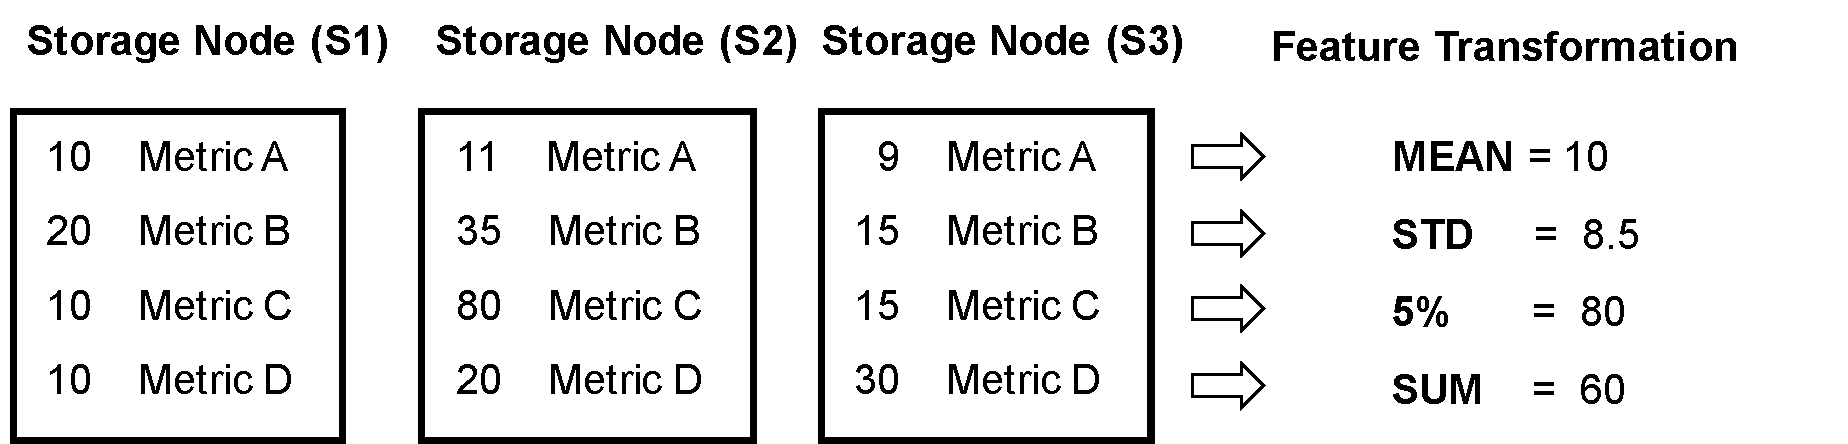
\includegraphics[width=0.9\textwidth, keepaspectratio]{figures/features.pdf}
\caption{Four statistical features used in Inside-Out to capture load and internal status of a distributed storage system.  The numbers and metrics represent low-level performance data collected from storage nodes.}
\label{fig:feature_types}
\end{figure}


%\subsubsection{Handling the distributed system scenario}
\subsubsection*{Capture important features of a distributed storage system}
%
%One important characteristic of a distributed storage system is that it can expand or shrink on demand 
A distributed storage system can dynamically expand or shrink
according to demand.
The performance model has to capture the current 
scale of the deployment, the bottlenecks, and the average and variance in performance
of individual components of the distributed system. For each low-level system metric collected from 
various components of the distributed system, we use four statistical variables to characterize the behavior of a distributed system (see \myfigure{\ref{fig:feature_types}}). 
The statistical variable \textit{mean} and \textit{std} describe whether the impact of the workload is evenly distributed among 
storage components. The \textit{sum} variable represents the scale of the deployment, while the variable \textit{5\%} (top 5 percentile) captures the hot spot situations. 
The feature transformation from raw system metrics to these four statistical values also allows Inside-Out to apply 
the uniform input format for developing performance models for distributed systems at different scales.

\subsection{Feature Selection}
\label{sec:non-deterministic}

In this work, we collect low-level performance metrics
from two components of Ceph
namely monitor (MON) and Object Storage Daemons (OSD).
We use \emph{dstat}, a monitoring tool to collect resource statistics,
to collect 32 low-level performance metrics in total.
These measurements are then transformed using the process described in \myfigure{\ref{fig:feature_types}} (refer to Section~\ref{sec:data_preprocessing} for more details).


Selecting the ``right'' features from high dimensional data
is a challenging task because
as computation complexity increases, prediction accuracy may decreases
~\cite{guyon2003introduction, Saeys12007}.
Furthermore, for our case, the right feature set is not always the identical.
Table \ref{tab:challenge_feature_selection} shows the \emph{model accuracy} of different learning methods when modeling 
read throughput. 
%\chin{
%verified with $10$-fold cross validation.
%}
We see that all learning methods achieve high model accuracy
even though they choose different features. 
The model accuracy was obtained using $k$-fold cross validation (\textit{k}=10),
a common technique for assessing model accuracy. 
The training data is partitioned into $k$ disjoint sets. 
A single data partition is used for validation purpose and the remaining $k-1$ partitions are used for training data.
Although all models yield good model accuracy, they perform poorly and inconsistently when the storage environment changes. 
In \myfigure{\ref{fig:challenge_generalization}},
we show the prediction accuracy under
%we show prediction accuracy when we make
three types of changes in the storage environment---increase in the size of the distributed 
storage system, read workload and individual storage IO request size.
These algorithms (discussed later in Section~\ref{sec:algorithm_selection}) do not yield consistent prediction accuracy any more. 
For example, Lasso can still predict well when workload has changed but Decision Tree cannot.
On the contrary, Decision Tree performs better than Lasso when the size of the storage system increases.
We suspect this is caused by the large feature space, which leads to the overfitting problem \cite{domingos2012few, hastie2005}.
Next, we manually remove most features and select only a few with a trial-and-error strategy.
As shown in \myfigure{\ref{fig:challenge_generalization}}, we see significant improvement in some cases, but not all. 
Since an SDS environment can change over time, it is important for our model to provide consistent prediction accuracy under system changes
such as software reconfiguration and cluster expansion.


\begin{table*}[t!]
\caption{Important features selected by different algorithms are not deterministic}
\centering
\label{tab:challenge_feature_selection}
%\begin{tabular}{|lll|lll|lll|lll|lll|}
%\resizebox{!}{.8\linewidth}{
\resizebox*{\textwidth}{!}{
\begin{tabular}{|lll|lll|lll|lll|lll|}
%\begin{tabularx}{1.0\linewidth}{|lXl|lXl|lXl|lXl|lXl|}

\hline
\multicolumn{3}{|c|}{\textbf{Lasso}}   & \multicolumn{3}{c|}{\textbf{Ridge}}   & \multicolumn{3}{c|}{\textbf{Elastic Net}} & \multicolumn{3}{c|}{\textbf{Decision Tree}} & \multicolumn{3}{c|}{\textbf{Random Forest}} \\
\hline
osd  & network.send  & sum  & \textbf{osd}  & \textbf{network.recv}  & \textbf{mean} & osd   & network.send   & sum    & osd    & disk.read       & sum    & osd    & disk.read       & sum    \\
osd  & disk.writ     & sum  & \textbf{osd}  & \textbf{disk.read}     & \textbf{5\%}  & osd   & disk.writ      & sum    & osd    & network.send    & sum    & osd    & network.send    & sum    \\
\textbf{osd}  & \textbf{cpu.sys}       & \textbf{sum}  & \textbf{osd}  & \textbf{load.15m}      & \textbf{std}  & osd   & disk.read      & sum    & osd    & network.recv    & sum    & osd    & disk.writ       & sum    \\
osd  & io.read       & sum  & osd  & network.send  & sum  & osd   & cpu.sys        & sum    & osd    & disk.writ       & sum    & \textbf{osd}    & \textbf{network.recv}    & \textbf{sum}    \\
osd  & vm.minpf      & mean & osd  & tcp.tim       & std  & osd   & tcp.lis        & sum    & \textbf{mon}    & \textbf{memory.buff}     & \textbf{mean}   & osd    & memory.cach     & sum    \\
\textbf{mon}  & \textbf{memory.used}   & \textbf{5\%}  & osd  & network.recv  & std  & osd   & io.read        & std    & osd    & cpu.sys         & sum    & osd    & memory.buff     & mean   \\
\textbf{mon}  & \textbf{memory.cach}   & \textbf{5\%}  & osd  & load.5m       & std  & osd   & io.read        & sum    & osd    & vm.alloc        & sum    & osd    & memory.buff     & 5\%    \\
osd  & tcp.lis       & sum  & osd  & cpu.idl       & sum  & osd   & vm.minpf       & mean   & osd    & vm.minpf        & 5\%    & mon    & io.writ         & sum    \\
osd  & io.read       & std  & osd  & cpu.wai       & sum  & osd   & io.writ        & mean   & \textbf{mon}    & \textbf{cpu.idl}         & \textbf{std}    & osd    & memory.buff     & sum    \\
osd  & io.writ       & mean & osd  & cpu.sys       & sum  & \textbf{mon}   & \textbf{memory.used}    & \textbf{sum}    & mon    & memory.cach     & sum    & mon    & vm.free         & sum    \\
\hline
\multicolumn{3}{|c|}{96.20\%} & \multicolumn{3}{c|}{96.60\%} & \multicolumn{3}{c|}{96.18\%}     & \multicolumn{3}{c|}{96.78\%}       & \multicolumn{3}{c|}{96.94\%} \\
\hline
\end{tabular}
%\end{tabularx}
}
\end{table*}



\begin{figure*}
    \centering
    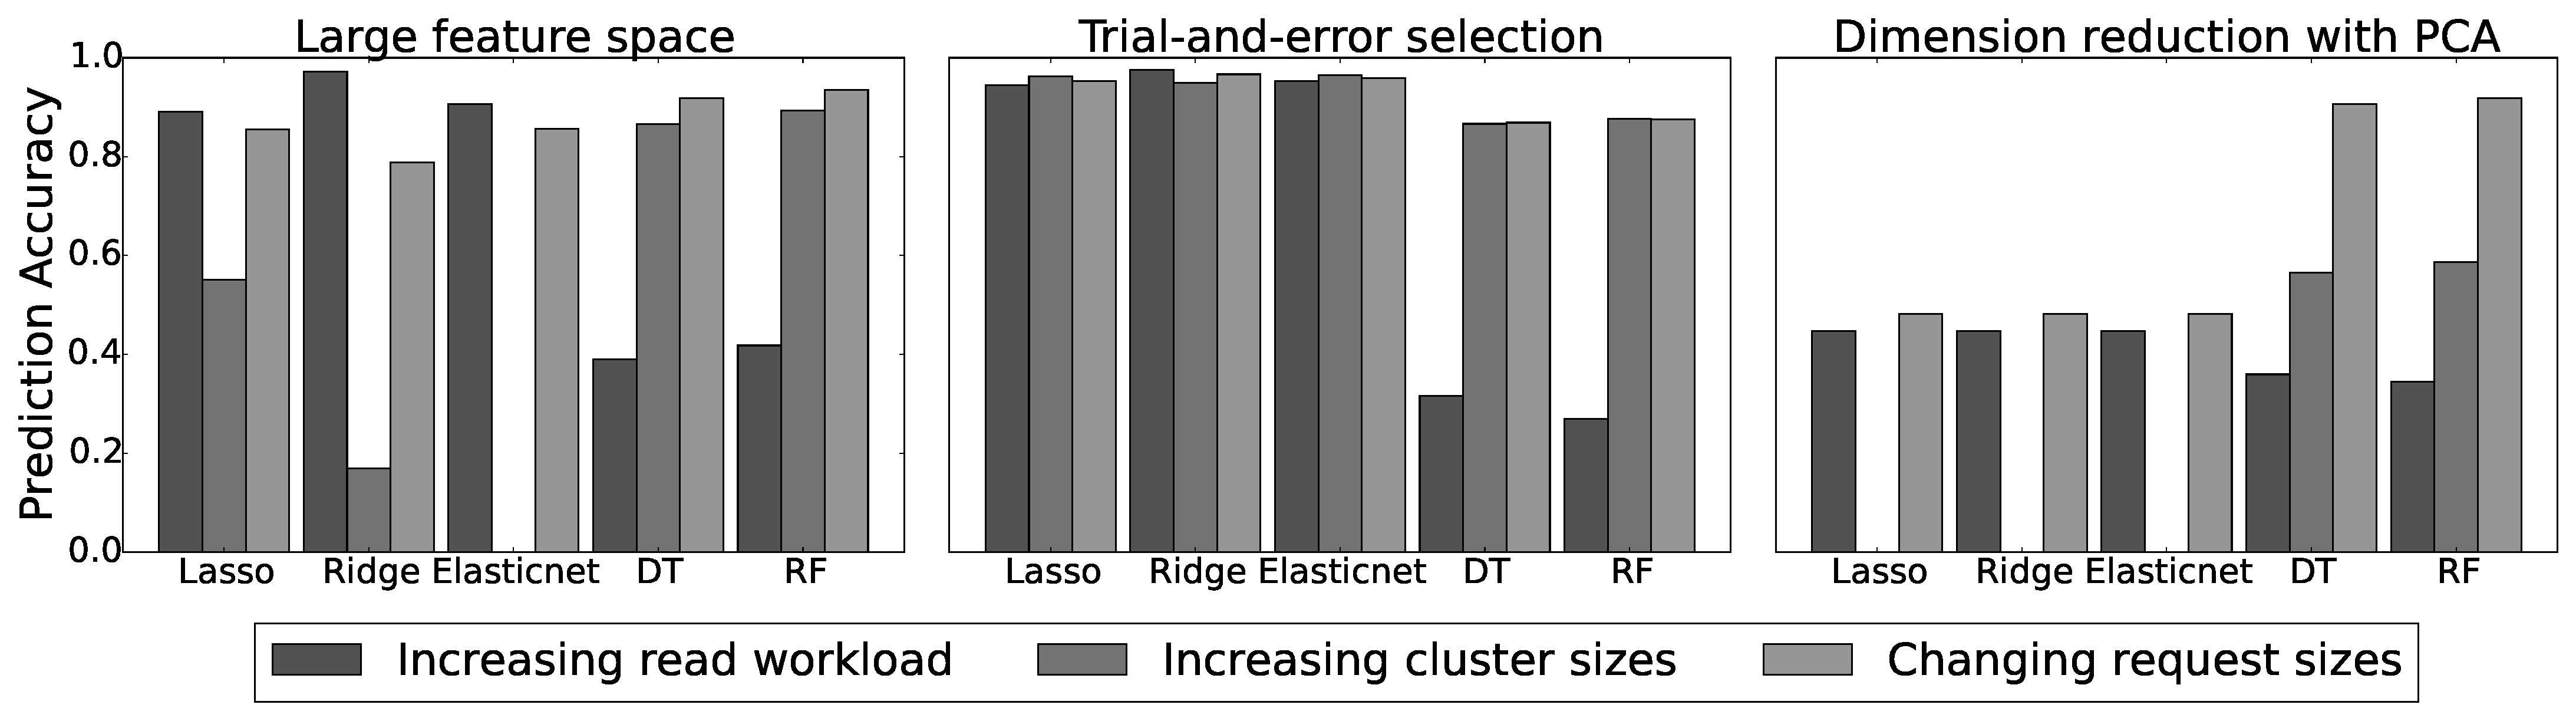
\includegraphics[width=1\textwidth]{figures/challenge_generalization_combined_horizental.eps}
    \caption{Prediction accuracy is inconsistent due to the large feature space.
    Learning methods fail to select the right features in some cases.
    Dimension reduction (PCA with 10 components) does not help in this case.
    In the trial-and-error case, we select a subset of metrics, e.g. \emph{mean(disk.read)}, \emph{sum(network.recv)} and \emph{std(cpu.usr)}.}
    \label{fig:challenge_generalization}
\end{figure*}

Although Hyperparameter tuning, model selection, and 
feature selection have been proposed as potential solutions, it is challenging 
to use them in practice, not to mention the complexity of automating this task. 
PCA (Principle Component Analysis) is another potential solution \cite{Shlens2003}.
PCA transforms original data into a lower dimension while keeping high fidelity.
However, PCA has several limitations. 
First, PCA is not scale invariant.
Not all performance metrics are comparable and therefore, there is no standard way to scale these metrics.
Second, PCA assumes Gaussian distribution in data points; however, many storage workloads have Pareto distribution \cite{Kim2010}.
Third, determining a good number of components is also a challenging task.
In our case, PCA does not address the problems.
In fact, \myfigure{\ref{fig:challenge_generalization}} shows that it can further degrade prediction accuracy.

\subsection{A Two-Level Approach}

Instead of performing feature selection or dimension reduction, we propose a generic two-step approach that can improve the consistency of prediction accuracy. 
In the first step, we use some heuristic methods to filter out irrelevant features.
Then, in the second step, we apply machine learning algorithms to build performance models with the reduced feature set.
The intuition behind this idea is that it is difficult to determine the most important performance features but it is relatively easy to eliminate unimportant features.
For example, the features which are not in the top 100 list after step one can be labeled as unimportant features.